% Drawing 154/07-19 -- folder 154, batch 07, archive page 130 (PDF page 131).
% Transcription: à gauche, dessins en couleur : deux disques tangents traversés de pseudo-droites rouges, un arc du bord hachuré en noir ; un disque vert traversé de pseudo-droites rouges, le bord marqué d'accolades $\alpha$, $\gamma$, $\beta$ ; un disque vert aux pseudo-droites rouges ; à droite, deux fois deux cercles, rouge et vert, qui se coupent en deux points
% Kind: disks crossed by red pseudo-lines; pairs of crossing circles. Method 2 (schematic redraw from the facsimile). Status: partial.
% Notes: Two tangent disks (light green rims, the left arc of the upper one thickened in black), a spindle running through both from the top of the first to the bottom of the second, four more red strands in the first and three in the second; the disk with the braces gamma (left), alpha (top) and beta (bottom), a spindle from top to bottom, three red strands and a dashed one; the lower disk with four red strands and five points on its rim; on the right two pairs of closed curves, one red and one light green, crossing each other twice. In the disks the strands are placed from a page view with their ends on the rim: their number is as read, the order of their crossings is approximate. The pencil hatching beside the black arc is left out. Redrawn 2026-11-12 (issue 128): to check again.
% Coordinates: 1 unit = 1 mm = 1/100 of the crop width (bbox in page fractions: [0.215, 0.14, 0.89, 0.5]).
% Redrawn by Claude (claude-fable-5-2), issue #128, 2026-11-12; not checked by a human; not compiled (no TeX in the session).
% Rights: reproduces part of the work -- behind RENDER_TRANSCRIPTS, never published by itself.
\documentclass[tikz,border=3pt]{standalone}
\usepackage{amsmath,amssymb}
\usetikzlibrary{patterns,arrows.meta}
\tikzset{Lg/.style={green!60!black!70}, Dg/.style={green!45!black}, Rd/.style={red!85!black}, pencil/.style={black!45}, struck/.style={black!35}, mpt/.style={circle,draw,inner sep=1.3pt}, pt/.style={circle,fill,inner sep=0.9pt}, opt/.style={circle,draw,fill=white,inner sep=1.1pt}}
\begin{document}
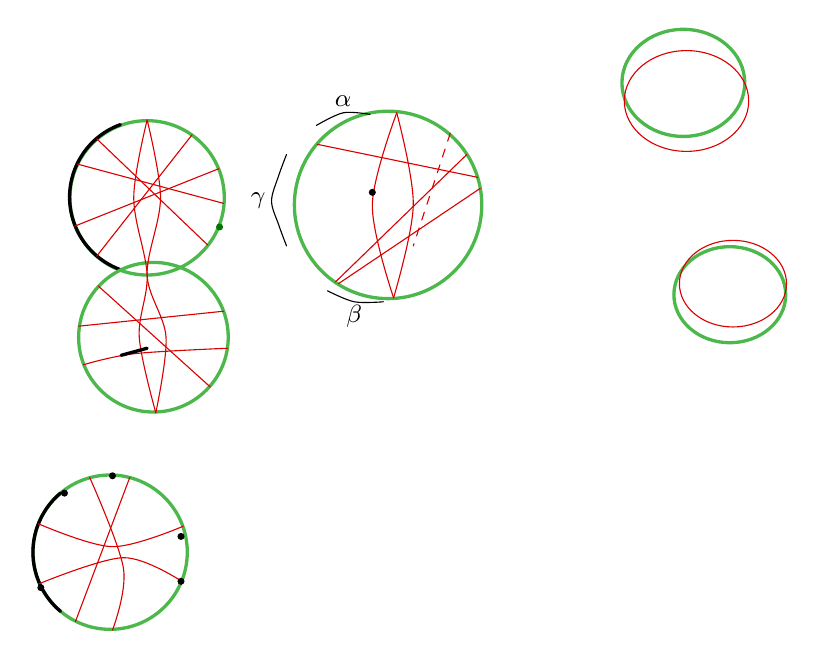
\begin{tikzpicture}[x=1mm,y=1mm,line cap=round,line join=round,font=\scriptsize]
\draw[Lg,very thick] (16.5,-18.1) circle[radius=9.8];
\draw[very thick] (13.1,-8.8) arc[start angle=110, end angle=250, x radius=9.8, y radius=9.8];
\draw[Lg,very thick] (17.3,-35.8) circle[radius=9.5];
\draw[Rd] plot[smooth, tension=0.55] coordinates {(16.5,-8.2) (14.8,-18.1) (16.5,-27.9) (15.5,-35.8) (17.6,-45.4)};
\draw[Rd] plot[smooth, tension=0.55] coordinates {(16.5,-8.2) (18.2,-18.1) (16.5,-27.9) (18.9,-35.8) (17.6,-45.4)};
\draw[Rd] (7.6,-13.8) -- (26.2,-18.8);
\draw[Rd] (7.3,-21.7) -- (25.6,-14.4);
\draw[Rd] (10.1,-10.6) -- (24.2,-24.1);
\draw[Rd] (22.2,-10.1) -- (10.1,-25.5);
\node[pt,Dg] at (25.7,-21.8) {};
\draw[Rd] (7.8,-34.4) -- (26.2,-32.5);
\draw[Rd] plot[smooth, tension=0.55] coordinates {(8.4,-39.3) (14.8,-37.9) (26.7,-37.2)};
\draw[Rd] (10.3,-29.3) -- (24.5,-42.1);
\draw[very thick] (13.2,-38.1) -- (16.5,-37.2);
\draw[Lg,very thick] (47.1,-19) circle[radius=11.9];
\draw[Rd] plot[smooth, tension=0.55] coordinates {(48.2,-7.3) (45.1,-19) (47.8,-30.8)};
\draw[Rd] plot[smooth, tension=0.55] coordinates {(48.2,-7.3) (50.3,-19) (47.8,-30.8)};
\draw[Rd] (38.1,-11.3) -- (58.5,-15.5);
\draw[Rd] (40.4,-28.8) -- (57.1,-12.6);
\draw[Rd] (58.8,-16.9) -- (40.8,-29);
\draw[Rd,dashed] (55,-9.9) -- (50.3,-24.2);
\node[pt] at (45.1,-17.4) {};
\draw plot[smooth, tension=0.55] coordinates {(34.2,-12.6) (33.2,-15.3) (32.3,-18.5) (33.2,-21.5) (34.2,-24.2)};
\node[inner sep=1pt] at (30.6,-18.5) {\small $\gamma$};
\draw plot[smooth, tension=0.55] coordinates {(38,-8.9) (41.4,-7.3) (44.8,-7.5)};
\node[inner sep=1pt] at (41.4,-5.8) {\small $\alpha$};
\draw plot[smooth, tension=0.55] coordinates {(39.4,-29.9) (42.8,-31.3) (46.5,-31.3)};
\node[inner sep=1pt] at (42.8,-33.2) {\small $\beta$};
\draw[Lg,very thick] (11.8,-63.1) circle[radius=9.8];
\draw[very thick] (5.5,-55.6) arc[start angle=130, end angle=230, x radius=9.8, y radius=9.8];
\draw[Rd] plot[smooth, tension=0.55] coordinates {(2.7,-59.5) (12.1,-62.4) (21.1,-59.8)};
\draw[Rd] plot[smooth, tension=0.55] coordinates {(2.8,-67.1) (13.5,-63.8) (20.9,-66.8)};
\draw[Rd] plot[smooth, tension=0.55] coordinates {(9.2,-53.6) (13.5,-65.2) (12.1,-73)};
\draw[Rd] (14.3,-53.6) -- (7.4,-71.9);
\node[pt] at (12.1,-53.4) {};
\node[pt] at (20.8,-61.1) {};
\node[pt] at (20.8,-66.8) {};
\node[pt] at (3,-67.6) {};
\node[pt] at (6,-55.6) {};
\draw[Lg,very thick] (84.6,-3.5) ellipse[x radius=7.8, y radius=6.8];
\draw[Rd] (85,-5.8) ellipse[x radius=7.9, y radius=6.4];
\draw[Lg,very thick] (90.5,-30.4) ellipse[x radius=7.1, y radius=6.1];
\draw[Rd] (90.9,-29) ellipse[x radius=6.8, y radius=5.5];
\end{tikzpicture}
\end{document}
